\documentclass[11pt,twoside]{report}
\usepackage{preamble}
\graphicspath{{../img/ch3/}}
\setcounter{chapter}{3}



\begin{document}

\chapter{Observing Zebrafish in 2D}
\label{chapter:fish_2d}



\epigraph{
They generally do not cause any injury, are said to suddenly appear and surprise people, and are a comparatively harmless type of yōkai.
}{Wikipedia: Hitotsume-kozō}


In this chapter we will focus on the methodology to observe zebrafish, swimming in a quasi two dimensional environment. The system was chosen for technical conveniences, as the 2D movement of fish can be captured by a digital camera. In comparison, recording the 3D movement of fish is a harder task, which will be discussed in chapter~\ref{chapter:fish_3d} and appendix~\ref{chapter:multi_view}. The spatial distribution of the fish will be discussed as the result.


\section{Introduction}


The vast majority of the collective behaviour of fish were performed in a quasi--2D environment, where the fish were confined in a shallow water tank. The motions of the fish can be captured by digital cameras and analysed by tracking softwares.



Even though the videos of a group of moving fish can be recorded easily, there are still technique challenges to extract the behaviour out of the experimental record. The difficult task is to identify of individual fish in a group.


\section{Methods}

Observing the fish in the lab includes the construction of the hardware (fish and fish tank), and the development of the software (fish tracking code). Both of them will be covered in the method section. The 2D tracking code will be reused in chapter~\ref{chapter:fish_3d} as basis for 3D tracking. 

\subsection{Fish and Apprautus}
\label{section:apprautus_2d}

\begin{SCfigure}
  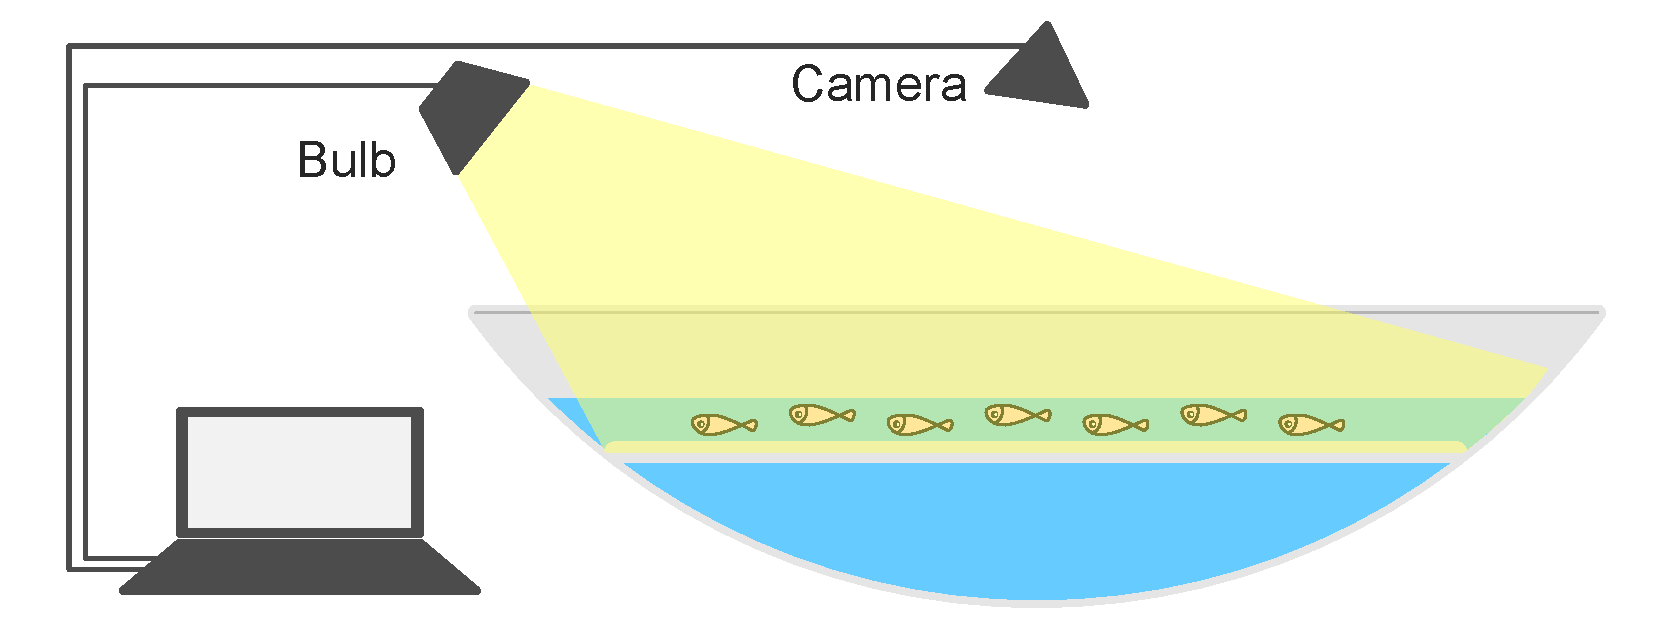
\includegraphics[width=\linewidth,outer]{apprautus-2d}
  \caption[Two dimensional fish tracking apprautus]{\label{fig:fish_apprautus_2d}
  The apprautus to track the movement fish in a quasi-2D environment. The camera is placed above the fish to capture the top view. A computer controls the recording process as well as the illumination.
  }
\end{SCfigure}

The adult zebrafish, whose age is over one year old, were used to carry out the experiment. Most small group experiments (N < 50) in this section was carried out in the fish facility in Bristol, and other experiments were carried out in room G59 in the HH Physics Laboratory in Bristol. The fish was fed three times a day, with natural day to night circles. The fish were living in their living tank before the experiments, with a density of 5 fish per litre of water. The water was filtered constantly, with a pH value close to 7 and the temperature close or above 25 °C.

Before each experiment, the fish were transferred from their living tank to the experimental environment, which will be referred to as the {\ot}. During the transfer, the fish were placed inside a temporary container, and then released into the {\ot}.

To make the fish stay in a quasi-2D environment, I placed the fish in a shallow tank, and placed a camera (Balser AC2040um) on top of the tank, as illustrated in Fig.~\ref{fig:fish_apprautus_2d}. A flat plate was placed in a bowl-shaped tank, creating a shallow water environment. The shape of the bowl is especially chosen for a 3D tracking task, which will be introduced in chapter \ref{chapter:fish_3d}.
I also used a smart light bulb (Kasa Smart Bulb, TP-Link) to control the brightness of the room with the computer.
\marginfootnote{It was worryingly easy to inject information to the smart bulb in 2020, and control its behaviour. All you need is a string of instructions, without any special encryption.}




\subsection{Metrical Rectification}
\label{section:metric_rectify}


The image and videos obtained from the camera have three drawbacks, preventing it from being an accurate measurement tool.
The first issue is the distortion of images caused by the camera lens.
In addition, the cameras should be orientated exactly perpendicular to the water surface, so that the captured images were from the top view. Such accurate orientation is difficult to achieve.
Finally, we also need to convert the unit of the image (pixels) to real life metrical units (e.g. meters).

To solve the problems, we need to \emph{calibrate} the camera, so that we know the distortion of the camera lens, the orientation of the camera, as well as the scale of objects in the images. Practically, I placed a chessboard (the calibration board) on the surface of the water. And the image of the calibration board will offer enough information to tackle the aforementioned issues. 

The distortion can be recovered with standard camera calibration methods from the computer vision community \cite{ma2005, hartley2003}. I used the functions from the ``opencv'' library. The distortion is described with the following model,

$$
\begin{aligned}
x_{\text {distorted }} &= x\left(1+k_{1} r^{2}+k_{2} r^{4}+k_{3} r^{6}\right) \\
y_{\text {distorted }} &= y\left(1+k_{1} r^{2}+k_{2} r^{4}+k_{3} r^{6}\right)
\end{aligned}
$$

\noindent where $r$ is the radius of the pixels in the image with respect to the optical centre. And $k_i$ values are the distortion coefficients, which will be used to recover the undistorted image.


The imperfect orientation can be fixed by the knowledge of the camera as well. Briefly, the same 2D plane in the 3D space, will form different projections with different cameras. These different 2D projections are related to each other by a projective transformation. Therefore, the same 2D plane for the fish in the imperfectly orientated camera are related to its counterpart, captured by the perfectly orientated camera. Such relation is termed as a \emph{homography}, and can be represented by a matrix
$\mathbf{H} \in \mathbb{R}^{3 \times 3}$. This matrix can be calculated easily with the knowledge of the camera, and here I followed the method proposed by \citeauthor{hartley2003} \cite{hartley2003}. The introduction of the projective transformation as well as the calculation of $\mathbf{H}$ are included in the appendix~\ref{chapter:multi_view}. With the rectified image, the scale can be recovered easily as we know the physical size of the calibration board.


Figure~\ref{fig:metric-rectify} shows an example of the metric rectification. Comparing the outline of boundary with/without distortion removed, it is clear that the raw image from the camera were distorted by the lens. The camera in the experiment were not perfectly perpendicular to the water surface, therefore the outline of the tank boundary appears to be an ellipse, because of the perspective transformation ($\mathbf{H}$). The ellipse were reverted back to a circle (right subfigure, Fig.~\ref{fig:metric-rectify}) after the rectification process.


\begin{SCfigure}
  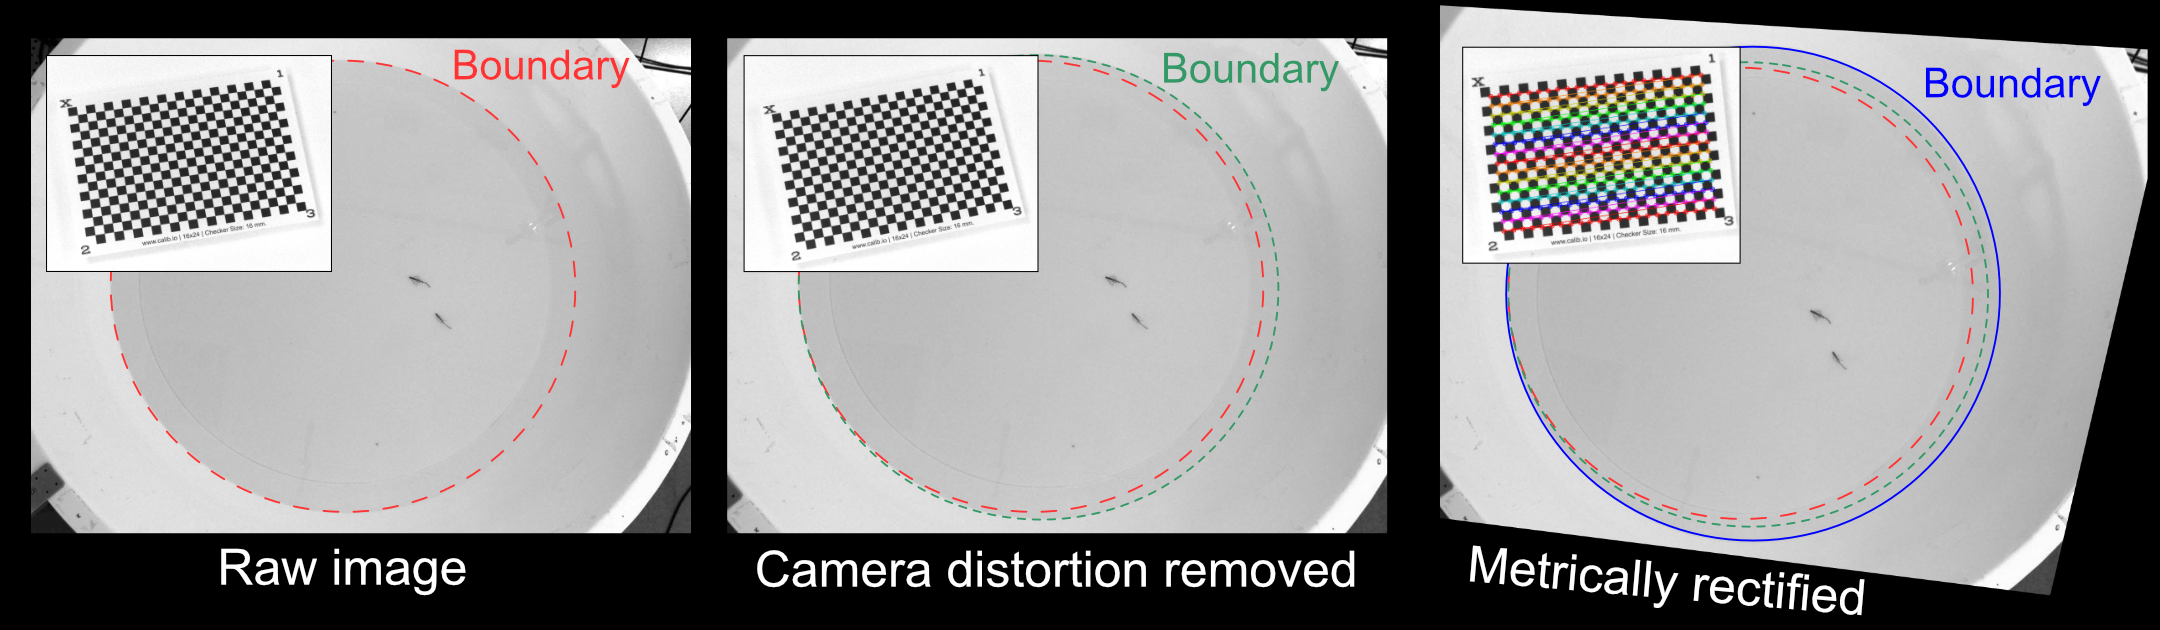
\includegraphics[width=\linewidth]{image-calib-2d.png}
  \caption[Metrical rectification of an image.]{
  	The process of metrical rectification. Left: the original image. Middle: the image where camera distortion being removed. Right: the metrically rectified image. The circular outline of the 2D boundary were outlined and overlaid, to stress the change of the image in different steps. The inserts in the figures correspond to the calibration pattern in each process.
  }
  \label{fig:metric-rectify}
\end{SCfigure}

\subsection{Image Processing}
\label{section:image_process}

The metrically rectified images of the fish contains the information about their behaviour.
To get useful information out of the image, still need to perform image processing, to extract the coordinates of the fish from the images.

In a normal image, the fish appear as a dark spot (Fig.~\ref{fig:metric-rectify}). 
Ideally, we want to work with images containing a collection of delta functions, where the pixel intensity in the centres of each individual fish is maximum, and the pixel intensities are zero everywhere else. Because extracting the coordinates of fish from such image will be a trivial task, as one only need to find the locations of non-zero pixels.

Even though it is possible to construct such transformation directly with machine learning based approaches \cite{newby2018}, it is still not a straightforward and easy task.
Therefore, I applied the traditional image processing methods, such as thresholding, blurring, and morphological operations, in this project.
As a result, I get a video where each fish have high pixel intensity values and the background intensity values are zero. Figure \ref{fig:2d_process} illustrate the result of the transformation. On the left side is the video recorded during the experiment, and the central image is the ``foreground'' after the image processing, where the background is removed.

The foreground videos of the fish were obtained after two  steps, the removal of the background and the removal of the noises. 
The background is defined as the temporal average of the image, since the fish are constantly moving while rest of the scene is static. In order to tackle the varying illumination conditions\marginfootnote{
The brightness level fluctuates even I keep the illumination setting unchanged in the laboratory. In a relatively dark ($\sim$20 lux) condition, those fluctuations could not be ignored.
}, I take a running average of a time--window, instead of calculating the overall average. The pixel intensity of the background at time $t$, of pixel $(i, j)$, can be written as

\begin{equation}
	B_{ij}(t) = \frac{1}{T} \sum_{\tau=t}^{t+T}{I_{ij}(\tau)}
\label{eqBG}
\end{equation}

\noindent where $I_{ij}(\tau)$ is the pixel intensity of the video at time $\tau$ in position $(i, j)$, and $T$ is the duration of the window, usually taken as 40 seconds. The difference between the background video and original video yields a foreground video, written as

\begin{equation}
	F_{ij}(t) = B_{ij}(t) - I_{ij}
\label{eqFG}
\end{equation}

\noindent and the order of the subtraction ensures the fish, originally appear darker in the video, would be represented by brighter pixels in the foreground video, shown in the centra image in Fig.\ \ref{fig:2d_process}. The subtraction result are often very noisy. To remove the noise, I applied gaussian filter to the foreground image, to smooth the sharp noises. Additionally, I applied the a combination of Ōtsu threshold and local gaussian threshold to separate the pixels belonging to the fish and other pixels. The Ōtsu threshold separate all the pixels into different groups to minimise the inter--group variance of the intensity distribution.

\begin{SCfigure}
  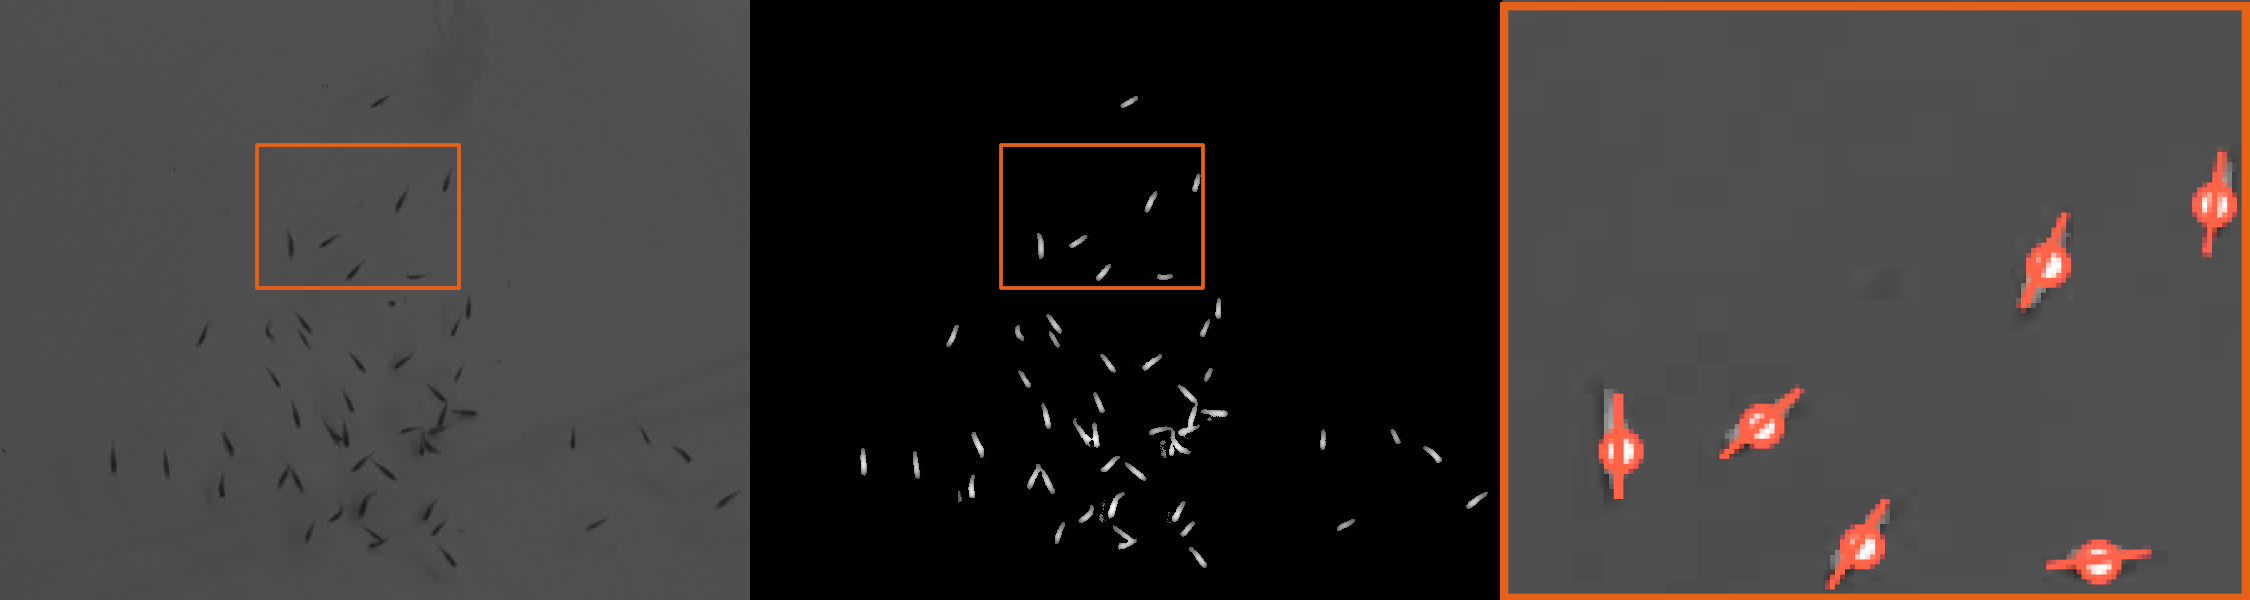
\includegraphics[width=\linewidth,outer]{2d-processing.png}
  \caption[Two dimensional image processing.]{Three successive image processing steps. Left: the image ($I_{ij}$)captured by the camera. Middle: the foreground Image $F_{ij}$. Right: the fish whose centres were labelled with a circle, and the orientation were labeled with a line.}
  \label{fig:2d_process}
\end{SCfigure}


\subsection{Extracting Features: General Idea}
\label{section:oishi}

From the processed video, it is to possible extract the features\marginfootnote{
In the computer vision community, people call the locations of objects ``features''. This slightly odd name roots in the 3D reconstruction problem, which will be discussed in the chapter~\ref{chapter:fish_3d}. Briefly, the 3D information can not be recovered from the background, like a purely white wall, where all the pixels have the same intensity value. Instead, some ``features'', with intensity gradients, are required\cite{ma2005}. Therefore, the locations of fish in images will be called ``features''. An alternative name would be ``positions/locations''. However, my selected is intensional, as I am talking about the ``feature'' of the photo, rather than a (3D) position of a fish.
}
in each frame that corresponds to the fish. In order to tackle the problem, we employed a method that not only capture the positions, but also the information of the fish orientations and body shapes. The basic idea is to calculate the cross--correlation between the image ($I_{ij}$) and a templated fish shape ($T_{ij}$), as the local maxima in the result would indicate the presence of a fish, because cross--correlation is a measure of similarity between signals.

For a fixed 2D fish template ($T_{ij}$), we can rotate it so that it contains $o$ different orientations. Calculating the cross--correlation of all the rotated templates, we can effectively get $o$ different results, and they can be concatenated into a 3D tensor (array), written as $C_{ijo}$. The tensor $C_{ijo}$ can be treated as 3D volumetric image. A local maxima in $C_{ijo}$, with coordinate $(i_m, j_m, o_m)$, indicates the presence of a fish at location $(i_m, j_m)$, with orientation $o_m$.


In addition, we are free to choose different templates for the fish shape, to capture the different postures. If $s$ different shapes were selected as templates, all of which were rotated into $o$ different orientations, then there will be $s \times o$ different templates. The cross-correlation of these templates with the image would yield a 4D tensor that can be shaped into $C_{ijos}$. A local maxima in the tensor, with coordinate $(i_m, j_m, o_m, s_m)$, represents a fish located at $(x_m, y_m)$, whose shape is like the $s_m$th template, with orientation $o_m$.


In summary, the cross--correlation between the image and the many templates yields a 4D tensor. This will be helpful for dealing with ``dense'' system, where the fish constantly overlap with each other. For the dense system, different fish will be separated into different regions in the shape--rotation space. For example, the overlapped fish pair in Fig.\ \ref{fig:fish_cross} was correctly labelled, by calculating the local maxima in the 4D tensor.


\begin{SCfigure}
  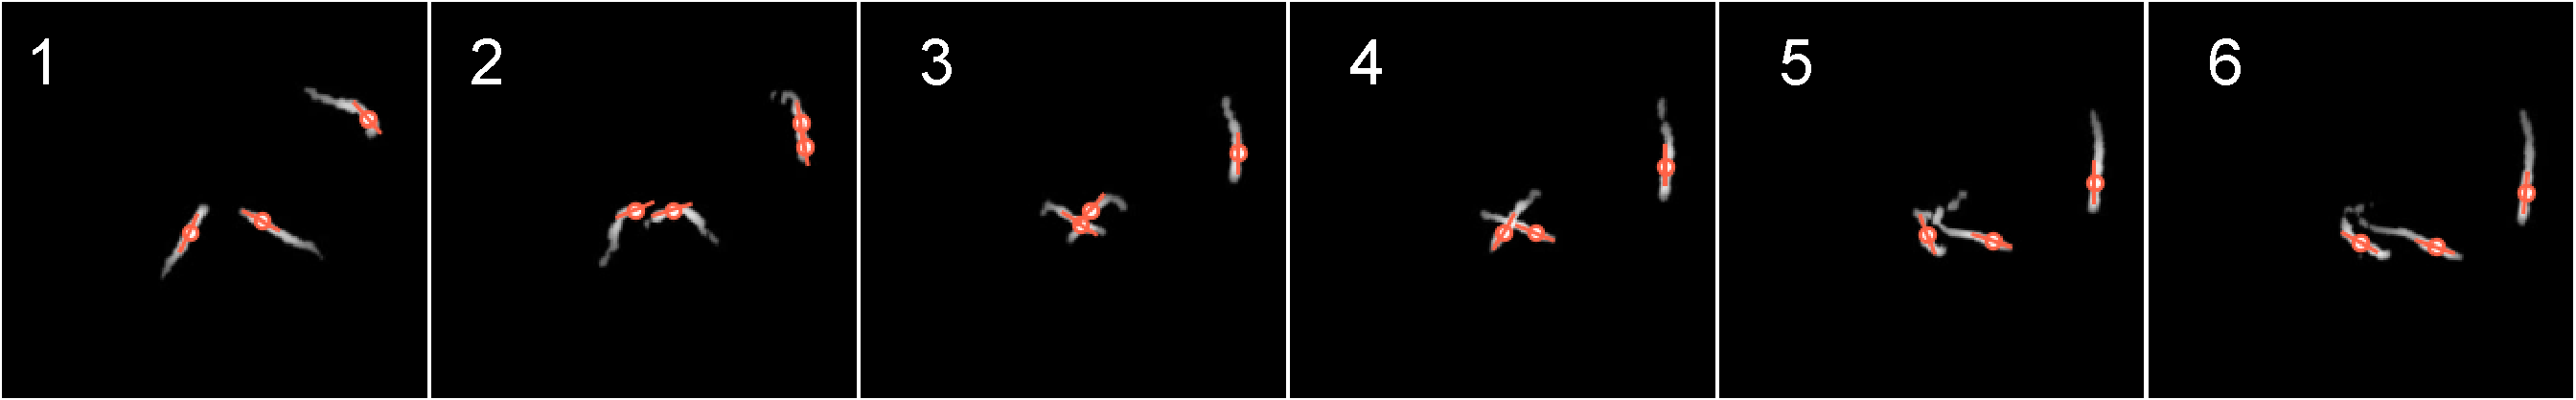
\includegraphics[width=\linewidth,outer]{cross-resolve}
  \caption{The movement of 3 fish in 6 successive frames. The crossed fish pair correctly labelled by the oishi feature detection algorithm.}
  \label{fig:fish_cross}
\end{SCfigure}


\subsection{Extracting Features: Find Templates}
\label{section:oishi_template}

The template of the fish should be representative examples of the shape of the fish. The unsupervised machine learning methods from the computer vision community are suitable in this situation \cite{goodfellow2016}. Typically, I used the following steps to find suitable templates to calculate the tensor $C_{ijos}$.

\begin{enumerate}
	\item Segment the individual fish and align the segmented images.
	\item Project all the segmented images to a space with reduced dimension.
	\item Find clusters for the data points in the reduced space, and the average of each cluster to be the template.
\end{enumerate}

The individual fish, defined as connected bright pixels, were segmented from the image ($I_{ij}$).
The orientation of the segmented fish were determined by the principle component analysis (PCA). These segmentations were then reoriented, so that its first principle axis align with the $x$ axis. The reoriented individual fish were then zero-padded to have the same shape, noted as $\mathbf{S} \in \mathbb{R}^{s \times s}$ where $s$ is the size of the padded images. Example of the segmented and aligned images were illustrated in Fig.~\ref{fig:fish_segment}. These images were collected over 1000 different frames, in a video of 2 swimming fish. A total of 2170 individual shapes were collected.


\begin{SCfigure}
  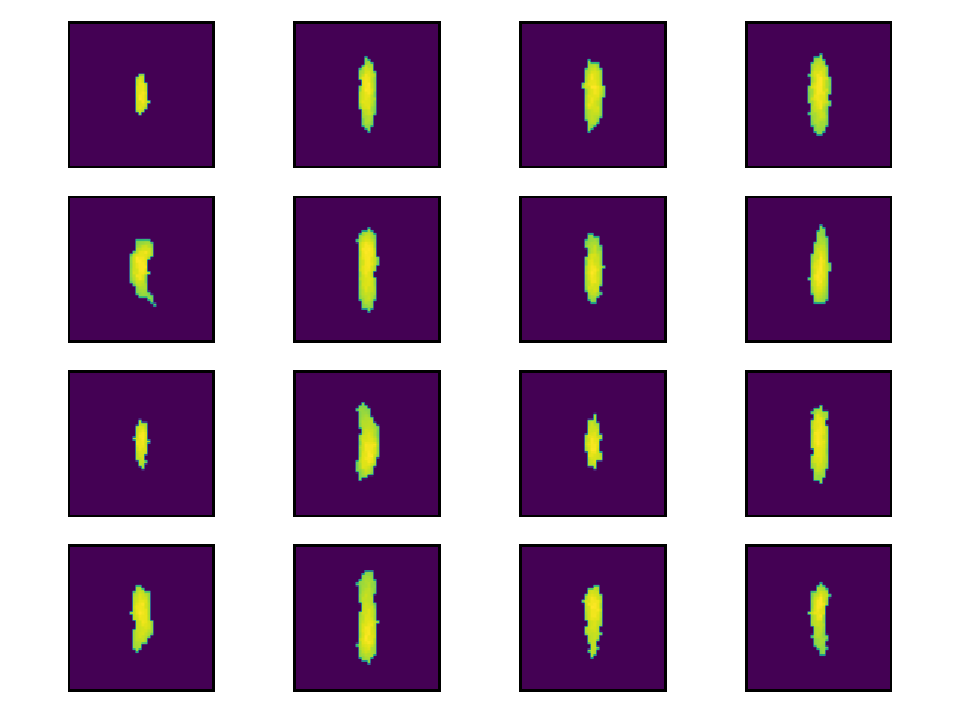
\includegraphics[width=0.75\linewidth]{segment_result_selection}
  \caption{The individual fish segmented from the images taken by the camera.}
  \label{fig:fish_segment}
\end{SCfigure}


The collection of segmented fish is a very large dataset. Typically, I use a small matrix of size $25 \times 25$ to stored each fish. This means each fish were be treated as a point in a 625 dimensional space.
The dimension of such images can be drastically reduced by PCA \cite{solem2012book}. Operationally, all of the $m$ images of individual fish were flattened
($\mathbb{R}^{s \times s} \rightarrow \mathbb{R}^{s^2}$),
and concatenate into a big matrix ($\mathbf{X} \in \mathbb{R}^{m \times s^2}$). For the dataset presented in Fig.~\ref{fig:fish_segment}, $m=2170$.

The singular value decomposition is performed on the dataset $\mathbf{X}$, following

$$
\mathbf{X} = \mathbf{U} \Sigma \mathbf{V}^T,
$$

\noindent where the matrices $\mathbf{U}$ and $\mathbf{V}$ contains all the left and right singular vectors, and the matrix $\Sigma$ contains all the singular values. The images ($\mathbf{X}$) were then project on the first $k$ axes ordered by their corresponding singular values. Effectively, the dimension of the matrix $\mathbf{X}$ were reduced from $m \times s^2$ to $m \times k$, forming a new matrix $\mathbf{X}_\text{red} \in \mathbb{R}^{m \times k}$. Each row in $\mathbf{X}_\text{red}$ described one fish.


\begin{SCfigure}
  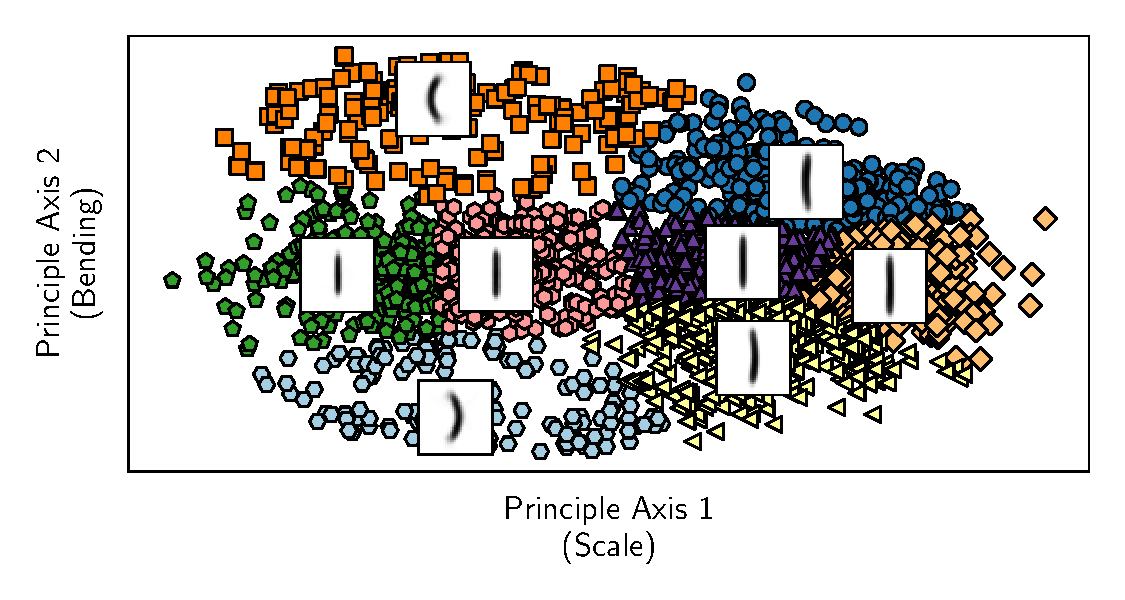
\includegraphics[width=\linewidth]{fish-pca-proj}
  \caption{
  	A collection of 2170 different fish shapes, projected onto the first two principle component axes. The data points were clustered using the K-means algorithm, into six different clusters, indicated by different marker styles. The average shape of each cluster were plotted in the inserted axes.
  }
  \label{fig:fish_pca}
\end{SCfigure}


Figure~\ref{fig:fish_pca} shows the average fish shape as well as the projection of all the segmented fish ($\mathbf{X}$) on the first two principle axes. The first principle axis (the $x$ axis of Fig.~\ref{fig:fish_pca}) roughly captured the scale of the fish, and the second principle axis (the $y$ axis of Fig.~\ref{fig:fish_pca}) captured the information about the bending of the fish. 
The overall distribution of those projected data can be understood by the fact that the same fish can have different distances and orientations, relative to the camera, so that their shapes will appear differently.
In addition, there is only bending shape when the fish appears bigger. This is because the small shape corresponds to a special orientation of the fish, where the bending is not distinguishable from the view of the camera.

With all the segmented fish being projected to low dimensional space, I use the k-means cluster algorithm to find representative cliques of the fish shapes. Briefly, different data points (different fish images in Fig.~\ref{fig:fish_segment}) will be assigned to different clusters. And the variance of points in the same cluster will be minimised, while the variance of points from different clusters will be maximised.

Each cluster corresponds to similar fish shapes. The average shape of different clusters were used as the template. The different scatters in Fig.~\ref{fig:fish_pca} shows the different clusters, and their corresponding average shapers were inserted. Here, the images ($\mathbf{X}$) were projected to a 5 dimensional space ($k = 5, \mathbf{X}_\text{red} \in \mathbb{R}^{2170 \times 5}$). And the overall 2170 points were separated into 6 different clusters. And the average shape of different clusters (the inserted subplots in Fig.~\ref{fig:fish_pca}) can be used as the templates to calculate the 4D tensor for tracking.

The number of clusters and the dimension of the reduced space ($k$) are free parameters, whose optimal values were hard to determine. Practically, I always set $k=5$, and separate the points into 8 different clusters, which yields good results for 2D tracking. The dimensional reduction method (PCA) and the clustering algorithm (K-means) can be changed to other tools with similar effects. For instance, it is possible to use non-linear dimensional reduction method such as isomap, and a gaussian mixture model to obtain different clusters. A detailed exploration of different methods is beyond the scope of this thesis.

The mapping from the image to the tensor, $I_{ij} \rightarrow C_{ijos}$ requires large amount of calculation, since a very large 4D tensor will be calculated. The speed can be significantly increased if the calculation were only performed on ``promising'' positions were a fish is likely to appear, and these positions corresponds to the local intensity maxima in the foreground image $F_{ij}$, defined in Eq.~(\ref{eqFG}). Practically, only a very small fraction of the tensor $C_{ijos}$ needs to be calculated. Such reduction of calculation can improve the calculation speed significantly.


\subsection{Extracting Features: Convolution Neural Network}
\label{section:cnn}

There are two steps in the image processing that can be improved in the image processing pipeline. The first one is the removal of background. In my current method, I calculated a rolling average of the entire video. The window size of the averaging operation is set by the user, which is very difficult to optimise because the video processing typically takes hours to finish. Practically, a rule-of-thumb number (600 frames) was applied. However, the fish in the video are very distinct from their background, and it is an easy task for people to spot the fish in a static image. This suggests a static image contains enough information to distinguish the foreground (fish) and background (tank). 

The convolutional neural network (CNN) is very suitable for carrying out both tasks at the same time, with far better efficiency. The overall data process introduced from section~\ref{section:image_process} to section~\ref{section:oishi_template}, is essentially a transformation from the image ($I_{ij}$) to a tensor ($C_{ijos}$). In addition, the information about the kernel is unnecessary in most cases, as we often only care about the orientation and location of the fish, rather than its shape. Hence, we need a model with the capacity to carryout the following transformations depending on our desired results:

$$
\begin{aligned}
I_{ij} &\rightarrow C_{ijos} 
&\textrm{location, orientation, and shape} \\[1ex]
I_{ij} &\rightarrow C_{ijo}\;(= \max_{s}{C_{ijos}})
&\textrm{location, and orientation} \\
I_{ij} &\rightarrow C_{ij}\;(= \max_{o}{C_{ijo}})
& \textrm{location} \\
\end{aligned}
$$

\noindent And we can generate a big dataset containing known $I_{ij}$ and its corresponding $C_{ijos}$, and make a CNN to learn the underlying rules for the transformation ($I_{ij} \rightarrow C_{ijos}$). If we need less information from the result, the targeted $C$ can be contracted, by taking the maximum value along the dimension of the unnecessary information.

As a proof of concept, a CNN model was built to carry out the transformation of $I_{ij} \rightarrow C_{ij}$. The training data for the network was generated from the existing tracking result $C_{ijos}$.
The model was built with popular framework tensorflow, and trained on Colab online platform provided by Google.
Fig.~\ref{fig:track_cnn} shows the output of a trained network. However, due to the limited time for me to optimise the training and network structure, the final CNN model did not improve the calculation accuracy nor the processing speed significantly. Nevertheless, the direction is prosing, and I think it is achievable to having the calculations so optimised that the tracking can be performed in real time.


\begin{SCfigure}
  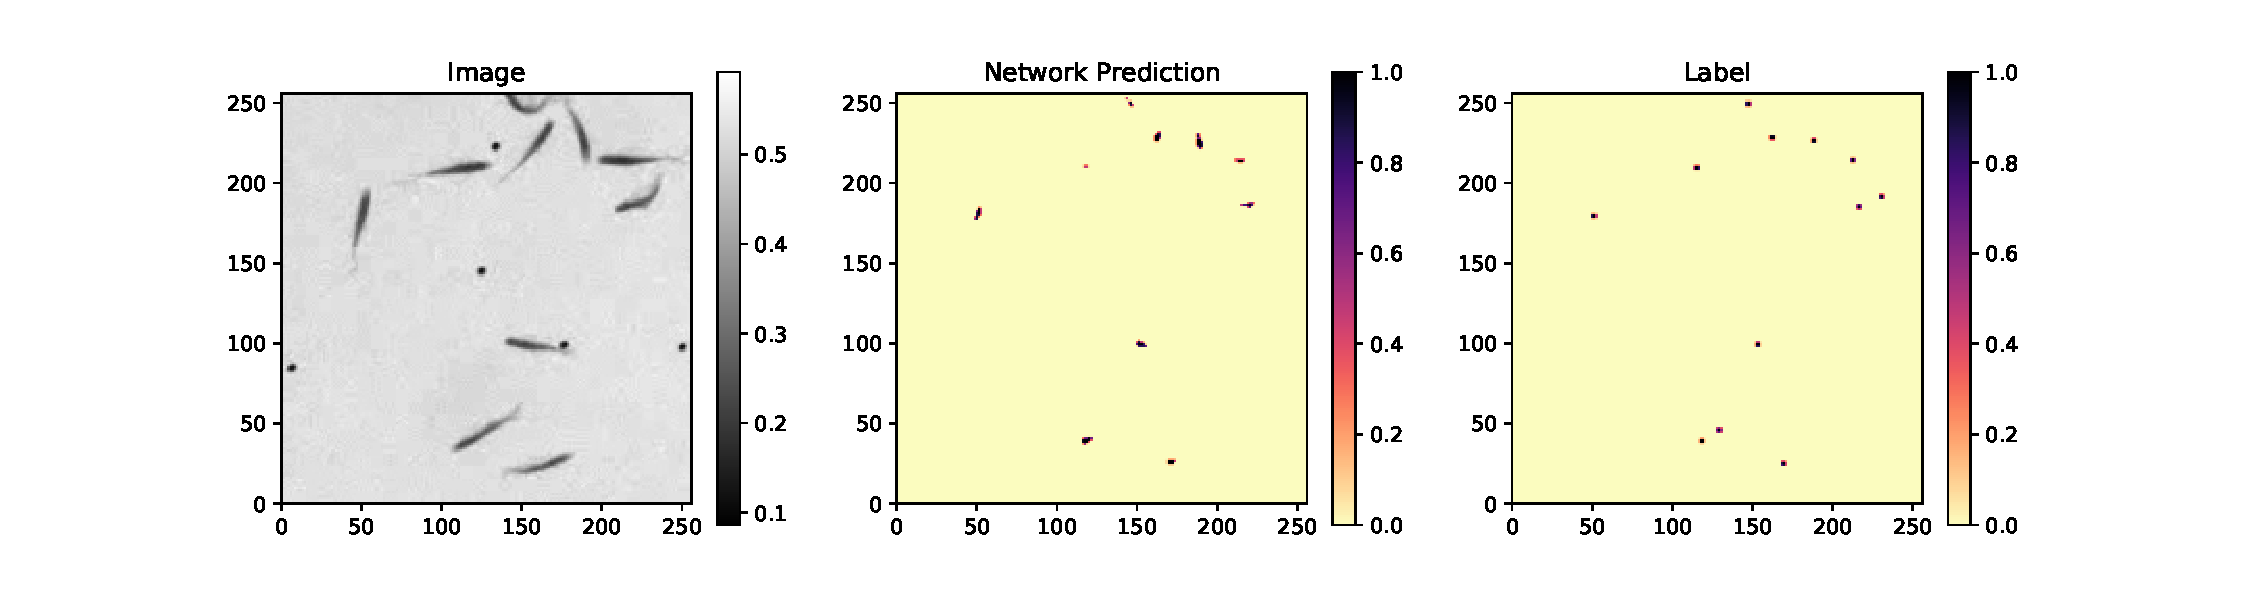
\includegraphics[width=\linewidth]{track-cnn}
  \caption{
	The tracking result of a convolutional network.
  }
  \label{fig:track_cnn}
\end{SCfigure}

\section{The 2D Spatial Distribution of Zebrafish}

In this section I will present the spatial distribution of zebrafish.

\subsection{A Single Fish}
\label{section:fish_1_2d}

Yushi: needs new data.

\subsection{A Pair of Fish}
\label{section:fish_2_2d}

The movement of 2 adult zebrafish were recorded. The result composed of 5 experiments, and each experiment lasts one hour.
The spatial distribution of 2 fish were shown in Fig.~\ref{fig:density_2d_fish_2} (left). It is clear that the fish were not uniformly distributed in the tank, which might also related to the environmental factor.

The pairwise distance of the 2 fish offered us the way the characterise their cohesion. If the fish were attracted to each other, they would stay close, and vice versa. The distribution of the pairwise distances were plotted in the Fig.~\ref{fig:density_2d_fish_2} (right).  


\begin{SCfigure}
  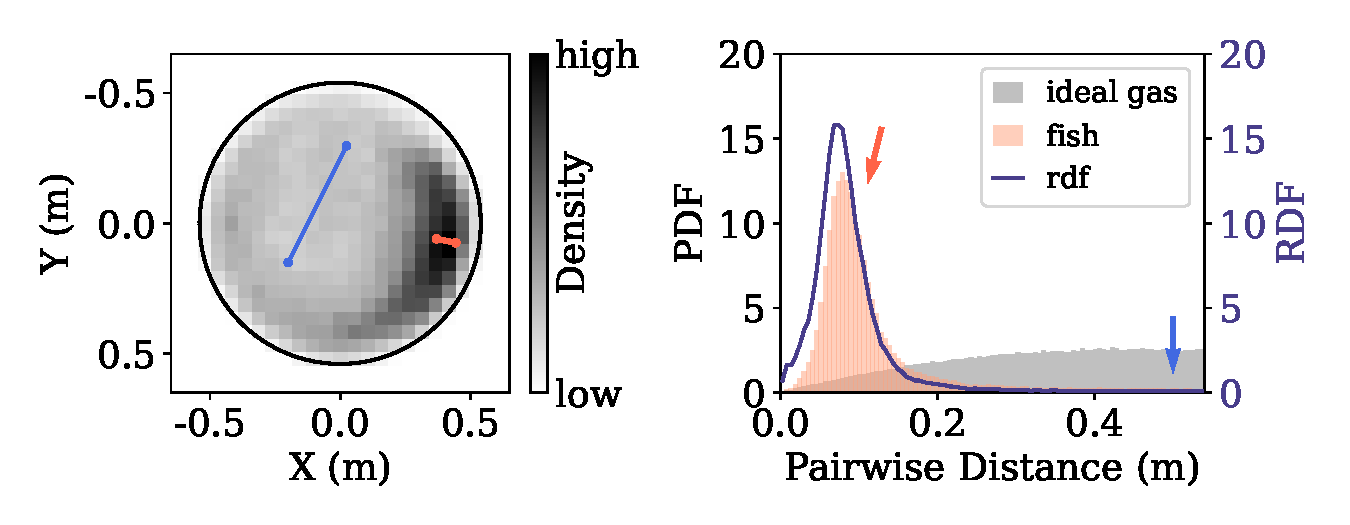
\includegraphics[width=\linewidth]{dist-2-fish}
  \caption[The 2D spatial distribution of two fish]{The spatial distribution of two adult zebrafish in a quasi 2D environment. Left: the joint distribution of the $X$ coordinates and $Y$ coordinates of the fish positions, with the shape of the boundary being highlighted. Right: the probability density function (PDF) for the distance between two fish. The PDF for the distance of 2 ideal gas, uniformly distributed in the tank, were also plotted. The ratio of the two PDFs were taken as the radial distribution function (RDF).}
  \label{fig:density_2d_fish_2}
\end{SCfigure}


\subsection{Three Fish}
\label{section:fish_3_2d}


\begin{SCfigure}
  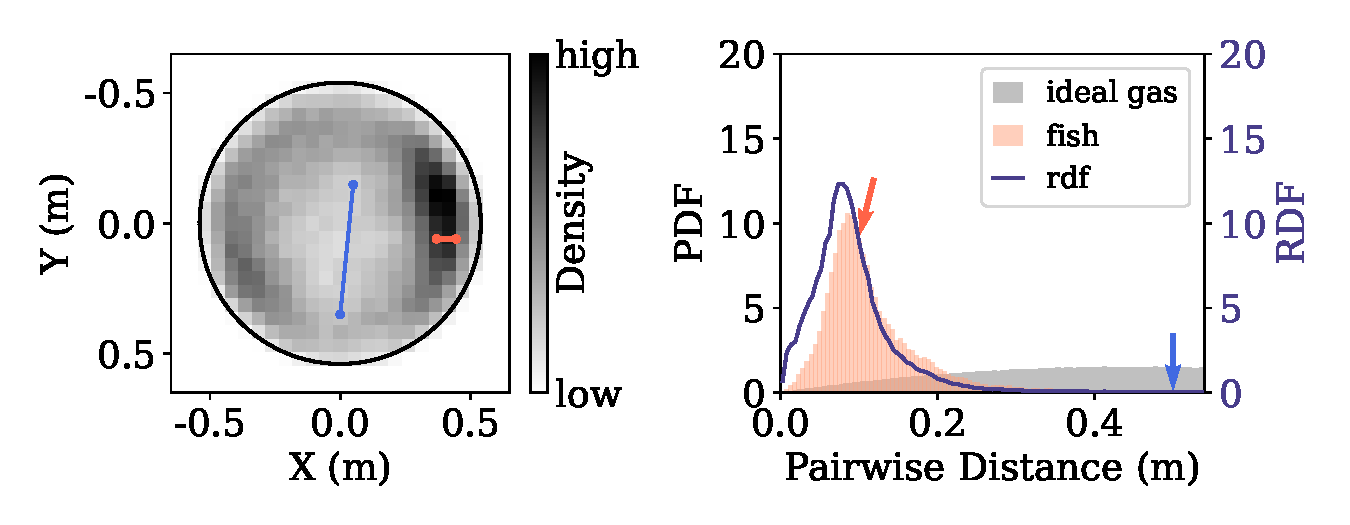
\includegraphics[width=\linewidth]{dist-3-fish}
  \caption[The 2D spatial distribution of three fish]{The spatial distribution of three adult zebrafish in a quasi 2D environment. Left: the joint distribution of the $X$ coordinates and $Y$ coordinates of the fish positions, with the shape of the boundary being highlighted. Right: the probability density function (PDF) for the distance between two fish. The PDF for the distance of 3 ideal gas, uniformly distributed in the tank, were also plotted. The ratio of the two PDFs were taken as the radial distribution function (RDF).}
  \label{fig:density_2d_fish_3}
\end{SCfigure}


\subsection{Many Fish}
\label{section:fish_many_2d}

\begin{SCfigure}
  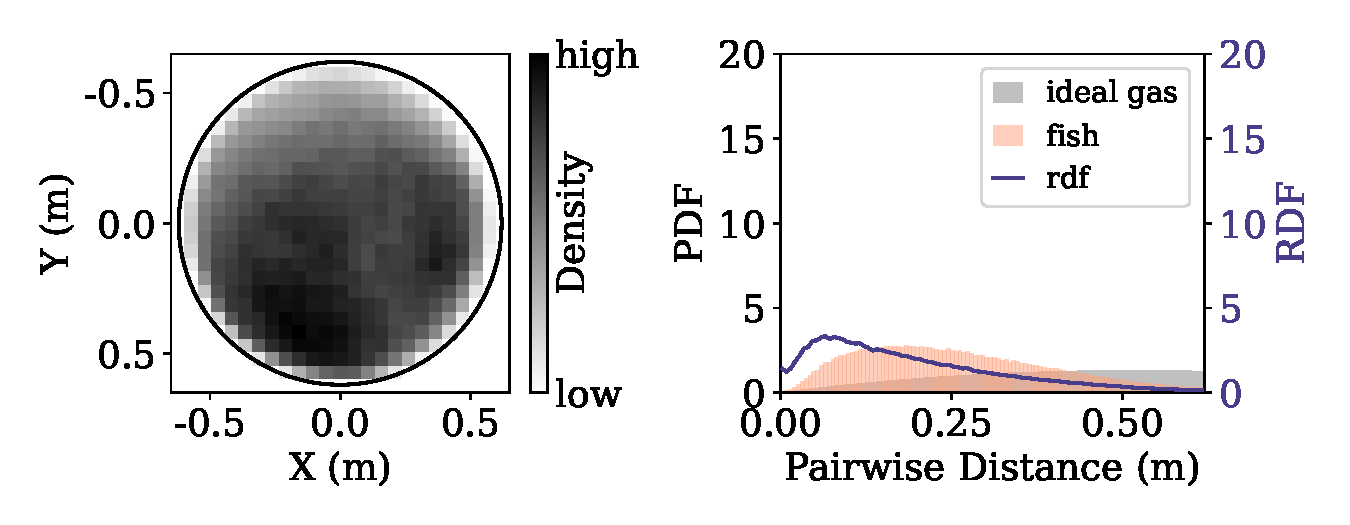
\includegraphics[width=\linewidth]{dist-50-fish}
  \caption[The 2D spatial distribution of 50 fish]{The spatial distribution of 50 adult zebrafish in a quasi 2D environment. Left: the joint distribution of the $X$ coordinates and $Y$ coordinates of the fish positions, with the shape of the boundary being highlighted. Right: the probability density function (PDF) for the distance between two fish. The PDF for the distance of 50 ideal gas, uniformly distributed in the tank, were also plotted. The ratio of the two PDFs were taken as the radial distribution function (RDF).}
  \label{fig:density_2d_fish_3}
\end{SCfigure}


\end{document}